\documentclass[runningheads]{llncs}
\usepackage{graphicx}
\usepackage{tabularx}
\usepackage{amsmath}
\newcommand{\code}[1]{\texttt{#1}}
\usepackage{xcolor}
\usepackage{fancyvrb}

\begin{document}

\title{COMP 472 Project 1 \\ Heuristic Search: Indonesian Dot Puzzle}

\author{Matteo Esposito\inst{1} \and
Matthew Liu\inst{2} \and
Kabir Soni\inst{3}}

\authorrunning{M. Esposito et al.}

\institute{40024121 \email{matteoesposito97@gmail.com} \and
40029238 \email{matthew.jx.liu@gmail.com} \and
40033019 \email{kabirsoni524@gmail.com}}

\maketitle   

\section{Introduction \& Technical Details}

This project was developed using python 3.7.4 64-bit.

\subsection{Files}

The file structure of our project is as follows:

\begin{table}
    \centering
    \caption{Files in project 1}\label{tab0}
    \begin{tabularx}{\textwidth}{|l|l|X|}
        \hline
        \textbf{Directory} & \textbf{Filename} & \textbf{Usage} \\ \hline
        \verb|out_dfs/| & * & Search and solution files for dfs \\ \hline
        \verb|out_bfs/| & * & Search and solution files for bfs \\ \hline
        \verb|out_a_star/| & * & Search and solution files for $A^{*}$ \\ \hline
        \verb|src/| & \verb|input_parser.py| & Input parsing functions, used to cast and convert input data into readable format \\ \hline
        & \verb|board.py| & Board class, used to represent the current puzzle\\ \hline
        & \verb|node.py| & Node class, used in all search algorithm and traversals \\ \hline
        & \verb|dfs.py| & Limited Depth-First Search algorithm implementation script \\ \hline
        & \verb|bfs.py| & Best-First Search algorithm implementation script \\ \hline
        & \verb|astar.py| & Algorithm $A^{*}$ implementation script \\ \hline
    \end{tabularx}
\end{table}

\subsection{Packages}

We used a total of 7 packages in our project, 5 existing, along with our 2 internal packages (board and node). 

\begin{enumerate}
    \item Existing 
    \begin{itemize}
        \item \verb|shutil| and \verb|os|: Folder and file management in the creation and deletion of output folders for our search and solution files. 
        \item \verb|time|: Runtime output. 
        \item \verb|math|: Updating and calculation of $h$ values (heuristic).
        \item \verb|copy|: Used to create deep copies of parent node when creating child nodes in the \verb|Board.touch()| method.
    \end{itemize}
    \item Internal
    \begin{itemize}
        \item \verb|board|: Class used to represent the puzzle 
        \item \verb|node|: Class that is used to represent the nodes in the tree traversal of all puzzle states involved in the search algorithms.
    \end{itemize}
\end{enumerate}

\subsection{Board and Node Classes}

The board class will take as input the puzzle in the form of a nested list, where each sublist is a row in the dot puzzle provided. The puzzle is converted into a nested list with the help of the \verb|parse()| method of the \verb|input_parser.py| script. It will then allow the search algorithms to call the goal test function to allow the search to terminate, as well as the print grid and touch methods to allow for well formatted printing of the puzzle and child node generation. \\

The node class will store the current move associated with the resulting puzzle, the puzzle itself (attribute 'state'), the node's parent puzzle. In the non-dfs cases, attributes g, h and f will also be used (cost, heuristic and evaluation function values) to help with the informed searches.

\section{Heuristic}

We defined 2 heuristics used by the Best-First Search and A* algorithms. They are as follows: 

\begin{equation}
% h_1(s) = 
% \Bigl\lfloor\dfrac{N^{(s)}_1}{5}\Bigr\rfloor\qquad
h_1(s) = \left\lfloor\dfrac{N^{(s)}_1}{5}\right\rfloor
\end{equation}

\begin{equation}
h_2(s) = N^{(s)}_1
\end{equation}

where $s$ denotes the current state and $N^{(s)}_1$ denotes the number of black dots in state $s$. Both heuristics count the number of black dots to estimate the cost of the cheapest path to the goal state. \\

In $h_1$, we make the simplifying assumption that any move can flip up to 5 arbitrary nodes. Under this assumption, the cheapest path to reach the goal would simply be to flip 5 black dots at each step until all dots are white. This heuristic is intuitive since any move by the player must flip 5 dots, but it fails to discriminate between states whose number of black dots have the same quotient when divided by 5. \\

For example, consider arbitrary states $s_1 =$ \code{111110000} and $s_2 =$ \code{100000000} represented in string form. Then both $h_1(s_1) = 1$ and $h_2(s_2) = 1$, even though $s_2$ is a more desirable state by number of black dots alone. \\

The main strength of $h_1$ is that it is an admissible heuristic. This is true because $h_1$ assumes any move flips $min(5,N^{(s)}_1)$ black dots and 0 white dots, whereas in reality a move would flip \emph{at most} 5 black dots, with the remaining dots flipped being white. In addition, $h_1$ is clearly a consistent heuristic, which makes the A* algorithm optimal under $h_1$ \cite{ref_2} \\

$h_2$, on the other hand, simply counts the number of black dots on the board. This heuristic fixes the problem $h_1$ had in discriminating between states that were clearly different. Going back to our example, $h_2(s_1) = 5$ whereas $h_2(s_2) = 1$. \\

However, $h_2$ is not an admissible heuristic, since it over-estimates the cost to reach the goal in at least 1 case, namely when the only 5 black dots on the board are arranged in a cross shape. Here, $h_2(s) = 5$ when the true cost is 1. \\

Both heuristics suffer from the fact that the composition of the board is never taken into account. That is, they both rely solely on the number of black dots to estimate the cost function. On the other hand, both $h_1$ and $h_2$ are extremely simple heuristics to calculate, making them intuitive and their evaluations fast. \\

\section{Difficulties}

\paragraph{Limited DFS} Initially, there were issues with the iterative implmentation of limited dfs. We were running into the issue where our closed list grew exponentially due to the branching factor which caused runtime issues. Taking a step back, we realized that a recursive implementation without the presence of an open and closed list would be satisfactory as we have a max depth parameter and are therefore not too severly affected by cycles in our search. \\

Next, since object-oriented design was a priority, we had to spend some time figuring out how exactly to structure the classes that would be involved in the project. We eventually chose to create a class for the puzzle (Board) and for the nodes which would be later used in the tree-traversals here and in other algorithm implementations.

\paragraph{Best-First Search} We began by implementing a recursive algorithm for Best First Search. However we soon realized that a recursive algorithm would not work properly as it does not keep track of visited and unvisited nodes. Therefore we were running into errors such as infinite recursion when nodes were being revisited back and forth. By implementing an iterative method, we were able to keep track of visited nodes with the presence of a closed list. This resulted in a search path of all unique nodes and better overall performance.

\paragraph{Algorithm $A^{*}$} Difficulties arose in the first implementation of algorithm A*. We initally decided to implement both algorithms recursively to combat the memory limitations of the iterative DFS. However, we needed a way to keep a running count of the number of nodes visited to date instead of only during the current call stack. \\

Passing in a \code{path\_length} variable to every call to \code{recursive\_a\_star()} and checking whether it hits a limit would only count the depth of a search down a given branch. Therefore, we ended up defining a simple \code{Counter} class that would be passed into every call to \code{recursive\_a\_star()} and count the number of calls. Using the \code{Counter} would avoid the counter resetting at the completion of each recursive call stack. \\

However, we soon realized that such an approach (without a closed list) would make the algorithm unable to distinguish between new and recurrent states, causing loops or repeated visits to certain states. It was ultimately decided that an iterative algorithm would perform much better, since the closed list is only limited by a constant $max_l$.

\section{Result \& Experiment Analysis}

\underline{Note:} To ensure consistency, all 3 search algorithms were tested on the same 3 puzzles as follows:

\begingroup\makeatletter\def\@currenvir{verbatim}
\verbatim
    1001 
    111001011
    1010010111001010
\end{verbatim}

\subsection{Limited Depth-First Search}

\begin{table}
    \centering
    \caption{Limited dfs runtimes as a function of the puzzle characteristics}\label{tab1}
    \begin{tabular}{|c|c|c|c|}
        \hline
        \textbf{Puzzle size} & \textbf{Max depth} & \textbf{Runtime} & \textbf{Average memory used} \\
        \hline
        2x2 & 4 & $\sim$ 0.002 seconds & 21.72MiB \\ \hline
        3x3 & 7 & $\sim$ 45.5 seconds & 36.44MiB \\ \hline
        4x4 & 15 & $\sim$ 71.6 seconds & 36.7MiB \\ \hline
    \end{tabular}
\end{table}

Compared to the other, informed search algorithms, we expect limited dfs to be the worst performer from a memory usage and time standpoint due to its uninformed nature. This search is also not complete, in that it is not guaranteed to find a solution. Since it is an exhaustive, recursive and stack based search, given branching factor $b$ and depth limit $l$, we have a time complexity of $O(b^l)$ and a space complexity of $O(bl)$. \cite{ref_2} \\

DFS will search every single node on the tree of child nodes generated from the root puzzle, which makes it very inefficient when compared to the quicker runtimes of the informed searches. (See appendix B)\\

Using the \verb|memory-profiler| module, which monitors memory consumption of a process \cite{ref_1}, we were able to generate memory usage charts of each of our serach algorithms. We notice that after the initial linear increase in memory usage (due to the I/O and parsing methods prior to the recursive dfs call), we have an average memory usage of 21.72, 36.44, and 36.7MiB for each puzzle respectively, which is greater than any of the other implementations for each of the puzzles. (See Appendix A)

\subsection{Best-First Search}

We compared the results and performance of both heuristics for BFS on all 3 test cases. \\

For the first test case, performance for both heuristics are very similar in terms of memory consumption and time. Both offer exact same solution paths, but different search paths. The first heuristic offers a more random search path for this small test case, but with similar performance, it makes it more desirable as it is an admissible heuristic. \\

For our second case, h2 manages to find the solution under 100 nodes, whereas h1 requires to search more just under 150 nodes. For the first heuristic, all nodes searched after the root have equal heuristics of 1, resulting in a again, a random search path, but for a more difficult puzzle. Therefore, h1 spent too much time visiting irrelevant nodes. H2 constantly attempts to minimize the number of black dots, which resulted in a much shorter search path, along with less memory consumption and shorter time. \\

For the last case, surprisingly memory consumption and time was very almost identical. Looking back at our second test case, the same logic should have followed for even a 4x4 puzzle. However, this anomaly may have resulted in similar search paths due to the nature of this particular puzzle for having a simple solution.

\begin{table}
    \centering
    \caption{BFS runtimes and memory usage with $h_1$}\label{tab1}
    \begin{tabular}{|c|c|c|c|}
        \hline
        \textbf{Puzzle size} & \textbf{Max nodes} & \textbf{Runtime} & \textbf{Average memory used} \\
        \hline
        2x2 & 100 & $\sim$ 0.0012 seconds & 17.88MiB \\ \hline
        3x3 & 150 & $\sim$ 0.2809 seconds & 26.74MiB \\ \hline
        4x4 & 100 & $\sim$ 0.0088 seconds & 21.84MiB \\ \hline
    \end{tabular}
\end{table}

\begin{table}
    \centering
    \caption{BFS runtimes and memory usage with $h_2$}\label{tab2}
    \begin{tabular}{|c|c|c|c|}
        \hline
        \textbf{Puzzle size} & \textbf{Max nodes} & \textbf{Runtime} & \textbf{Average memory used} \\
        \hline
        2x2 & 100 & $\sim$ 0.0615 seconds & 19.81MiB \\ \hline
        3x3 & 150 & $\sim$ 0.0876 seconds & 22.70MiB \\ \hline
        4x4 & 100 & $\sim$ 0.0121 seconds & 21.47MiB \\ \hline
    \end{tabular}
\end{table}

\subsection{Algorithm $A^{*}$}

We compare the results and performance of both heuristics for the iterative algorithm on our predefined test cases. \\

For our first test case, both heuristics perform identically, searching the same 4 nodes and reaching the same solution of 2 moves. Furthermore, we know from the properties of $h_1$ that this solution is optimal. \\

For our second case, only $h_2$ manages to find a solution while visiting less than $max_l=100$ nodes. This is likely due to the fact that $h_1$ does not actively try to reduce the number of black dots when searching. This, coupled with the larger number of states a 3x3 board presents (as opposed to the 2x2) meant that the $h_1$ implementation spent much of its time visiting many irrelevant nodes. \\

Our final test case shows this with a grid size of 4x4 as well. $h_1$ fails to find a solution under the maximum number of nodes while $h_2$ is successful. Again, $h_1$ visits too many nodes that don't lead to  a more favorable position. To illustrate this idea further, throughout the search path, $h_2$ never visits a state $s$ with $g(s) > g(s_0)$, where $s_0$ denotes the starting state. $h_1$, on the other hand, unable to discriminate easily between nodes, visits many states with $g(s) = g(s_0)$. (See appendix B)  \\

In order to analyse time and memory usage, we set an unlimited number of nodes to visit in our search. This ensures that we can accurately compare both heuristics by examining their asymptotic performance (i.e., letting the algorithms solve each grid). \\

The results are as follows:

\begin{table}
    \centering
    \caption{A* runtimes and memory usage with $h_1$}\label{tab1}
    \begin{tabular}{|c|c|c|c|}
        \hline
        \textbf{Puzzle size} & \textbf{Max nodes} & \textbf{Runtime} & \textbf{Average memory used} \\
        \hline
        2x2 & $\infty$ & $\sim$ 0.03 seconds & 15.0MiB \\ \hline
        3x3 & $\infty$ & $\sim$ 1.4 seconds & 17.5MiB \\ \hline
        4x4 & $\infty$ & $\sim$ 10.4 seconds & 18.7MiB \\ \hline
    \end{tabular}
\end{table}

\begin{table}
    \centering
    \caption{A* runtimes and memory usage with $h_2$}\label{tab2}
    \begin{tabular}{|c|c|c|c|}
        \hline
        \textbf{Puzzle size} & \textbf{Max nodes} & \textbf{Runtime} & \textbf{Average memory used} \\
        \hline
        2x2 & $\infty$ & $\sim$ 0.06 seconds & 13.5MiB \\ \hline
        3x3 & $\infty$ & $\sim$ 0.6 seconds & 17.2MiB \\ \hline
        4x4 & $\infty$ & $\sim$ 0.6 seconds & 17.3MiB \\ \hline
    \end{tabular}
\end{table}

We can see again that $h_1$ takes significantly more time than $h_2$ to solve more complicated grids, with the memory usage being modest accross all implementations. Again, detailed memory charts can be found in Appendix A.

\section{Team Responsibilities}

Due to there being three search algorithms that needed to be implemented and we are a group of three, we decided to take on an algorithm each. The breakdown of tasks were as follows:

\begin{enumerate}
    \item Matteo Esposito
    \begin{itemize}
        \item Input parsing functionality
        \item Node \& board class
        \item Limited Depth-First Search
    \end{itemize}
    \item Matthew Liu
    \begin{itemize}
        \item Node \& board class
        \item Algorithm $A^{*}$
    \end{itemize}
    \item Kabir Soni
    \begin{itemize}
        \item Best-First Search
    \end{itemize}
\end{enumerate}

\begin{thebibliography}{8}
\bibitem{ref_1}
memory-profiler 0.57.0, \url{https://pypi.org/project/memory-profiler/}. Last accessed 28 Feb 2020

\bibitem{ref_2}
S.J. Russel, P. Norvig: Artificial Intelligence: A Modern Approach. 3rd edn. Pearson, Harlow (1994)

\end{thebibliography}

\newpage

\section{Appendices}
\subsection{Appendix A - Graphs}

See following pages.

\begin{figure}
    \centering
    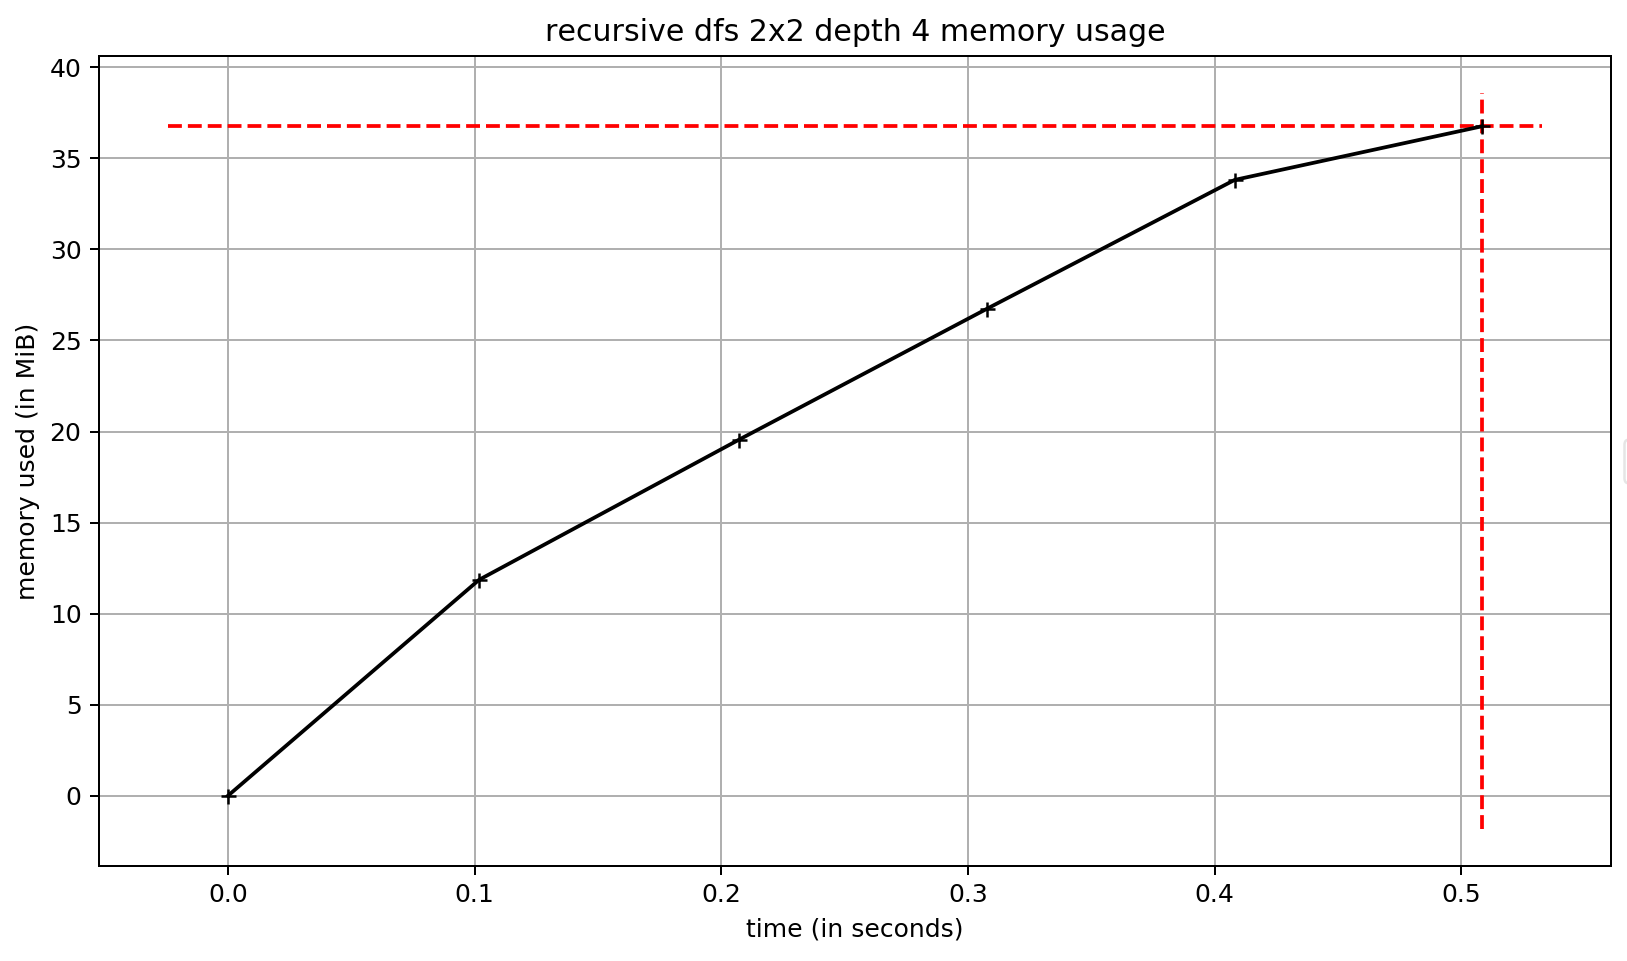
\includegraphics[width=10cm]{images/dfs-2x2.png}
    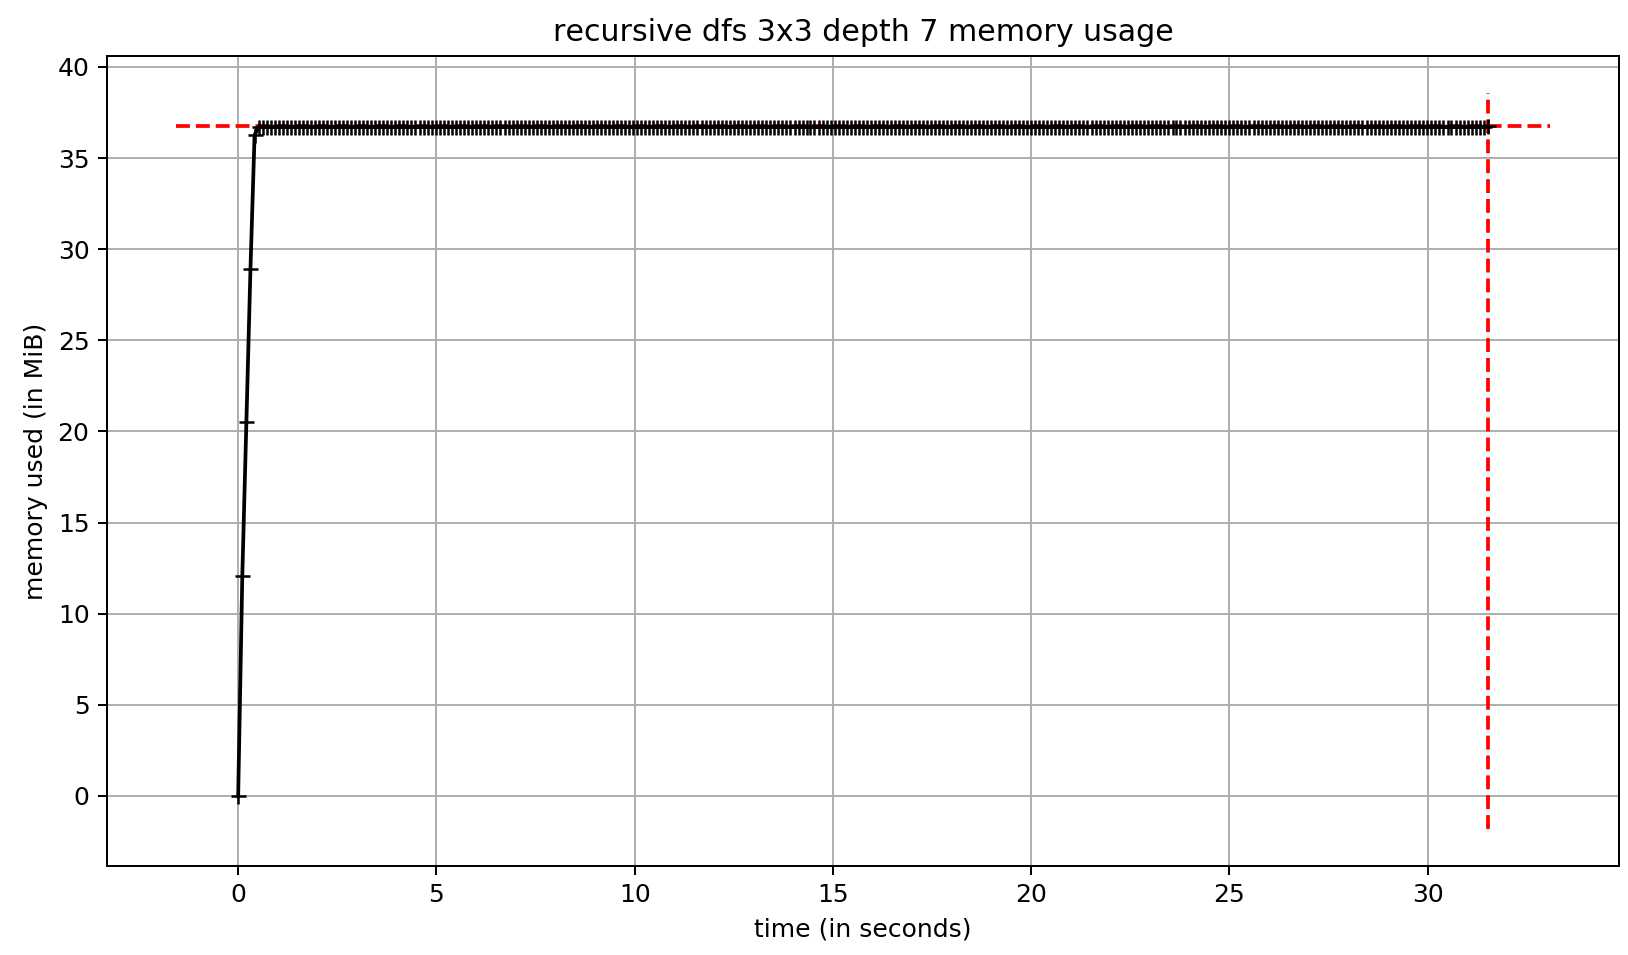
\includegraphics[width=10cm]{images/dfs-3x3.png}
    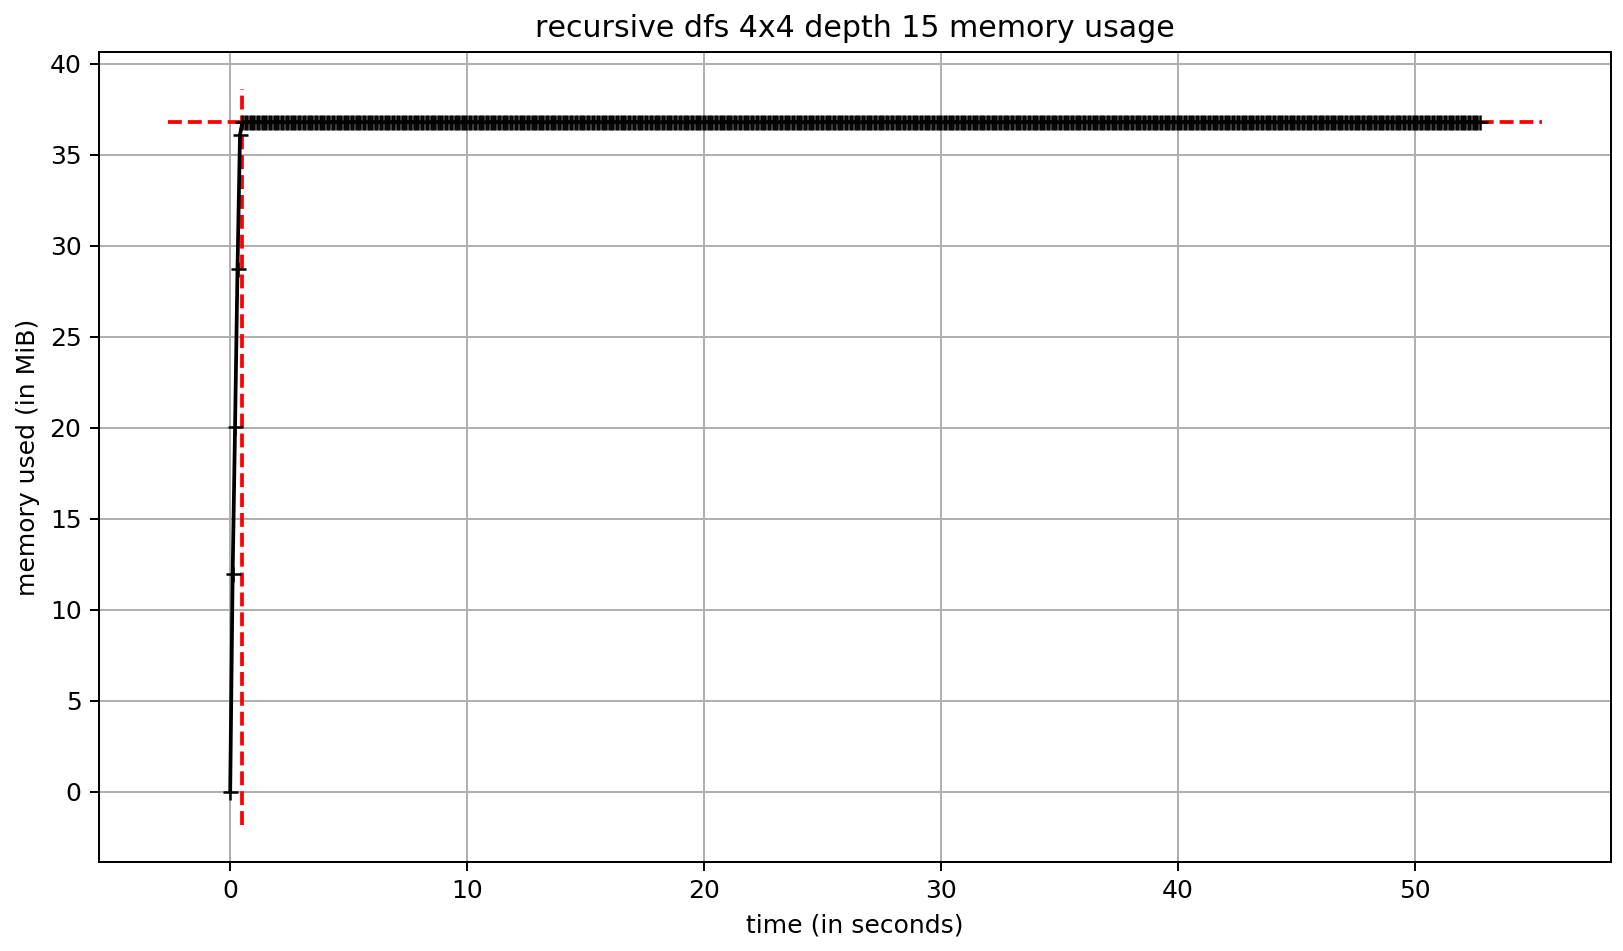
\includegraphics[width=10cm]{images/dfs-4x4.png}
    \caption{Memory usage of limited dfs} \label{fig1}
\end{figure}


\begin{figure}
    \begin{center}
        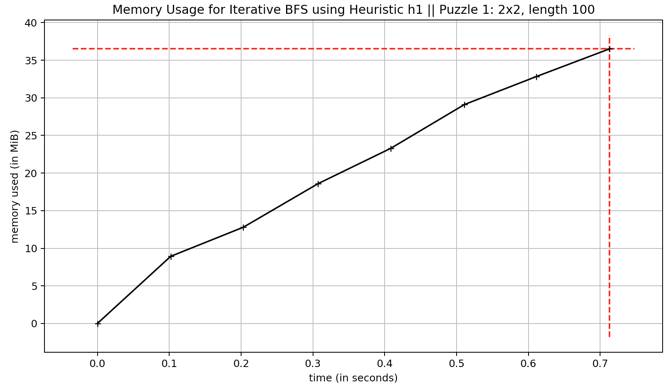
\includegraphics[width=10cm]{images/bfs-2x2-h1.png}
        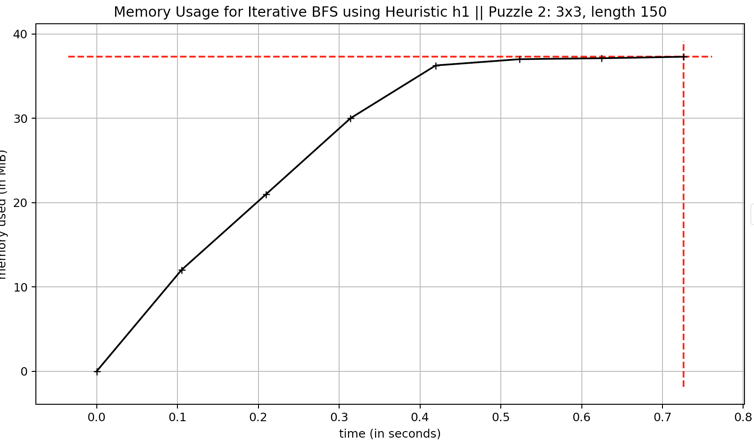
\includegraphics[width=10cm]{images/bfs-3x3-h1.png}
        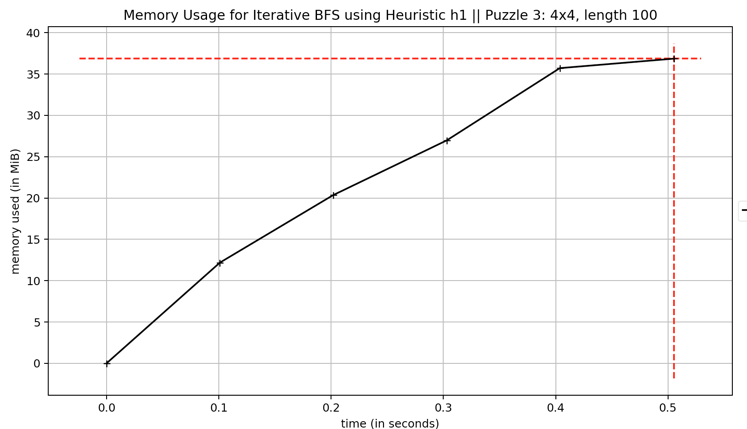
\includegraphics[width=10cm]{images/bfs-4x4-h1.png}
        \caption{Memory usage of A* under $h_1$} \label{fig2}
    \end{center}
\end{figure}
    
\begin{figure}
    \begin{center}
        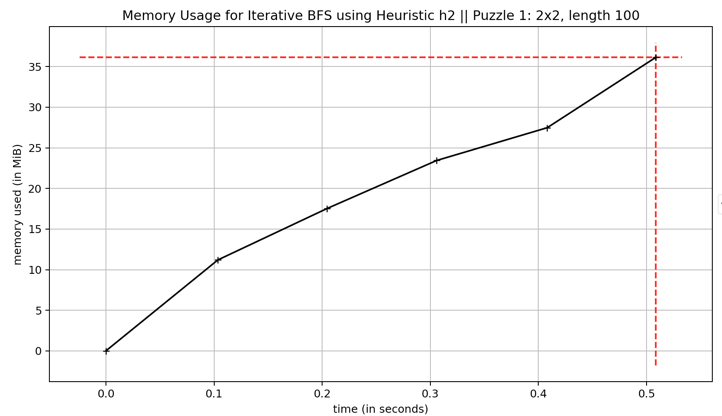
\includegraphics[width=10cm]{images/bfs-2x2-h2.png}
        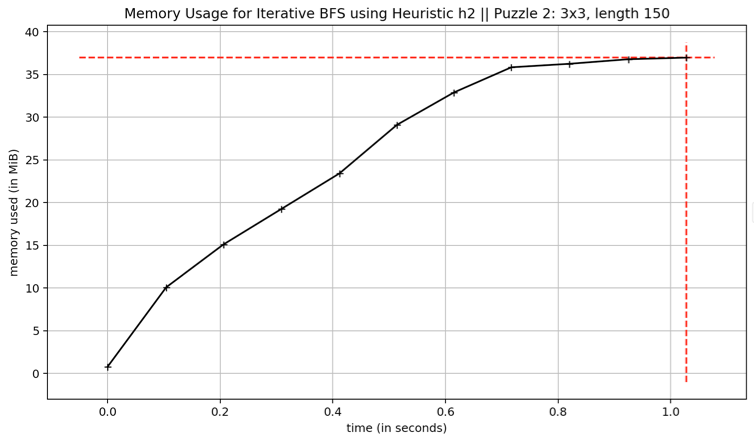
\includegraphics[width=10cm]{images/bfs-3x3-h2.png}
        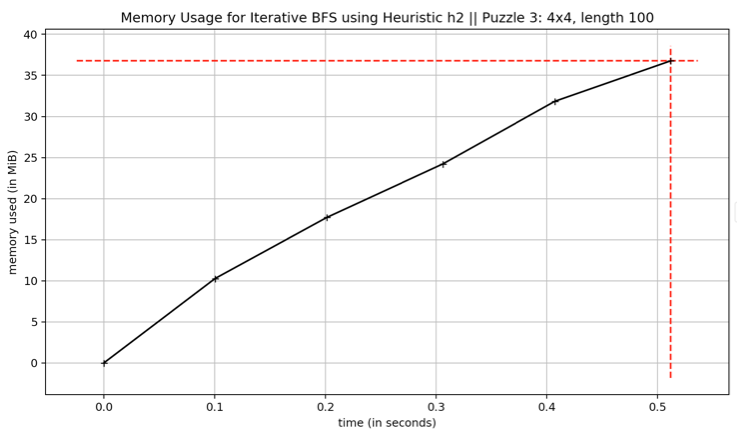
\includegraphics[width=10cm]{images/bfs-4x4-h2.png}
        \caption{Memory usage of A* under $h_2$} \label{fig3}
    \end{center}
\end{figure}
    

\begin{figure}
    \begin{center}
        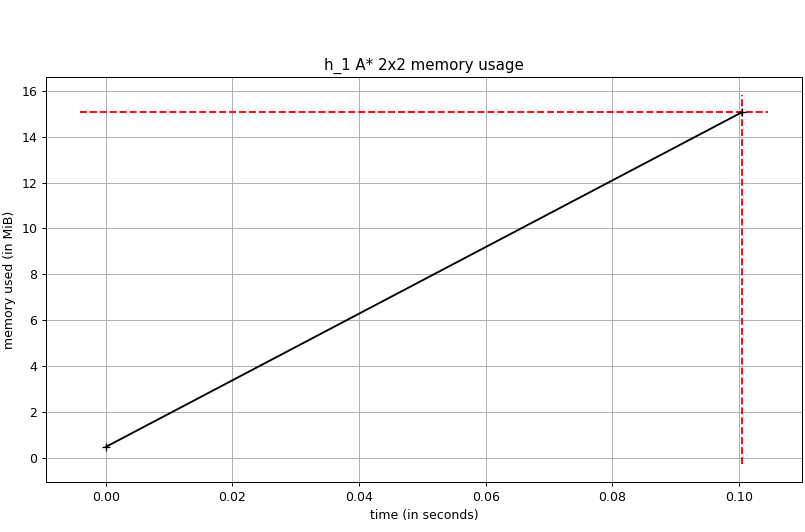
\includegraphics[width=10cm]{images/a_star_h1_2x2.png}
        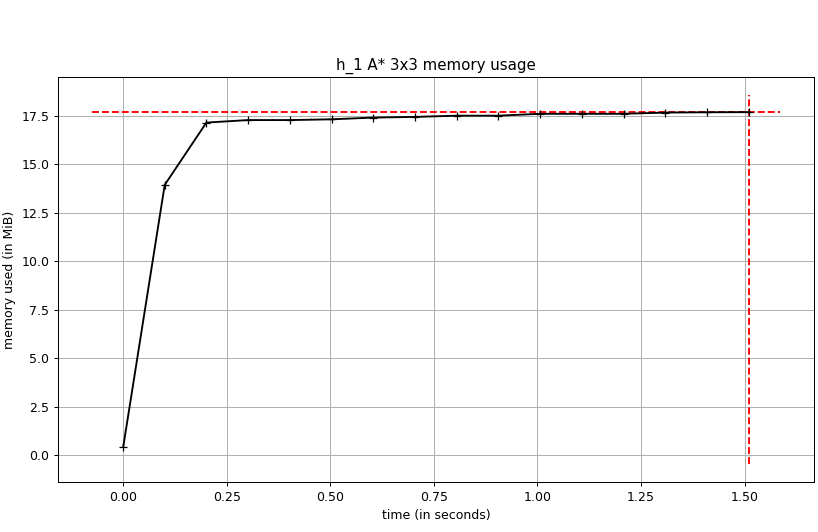
\includegraphics[width=10cm]{images/a_star_h1_3x3.png}
        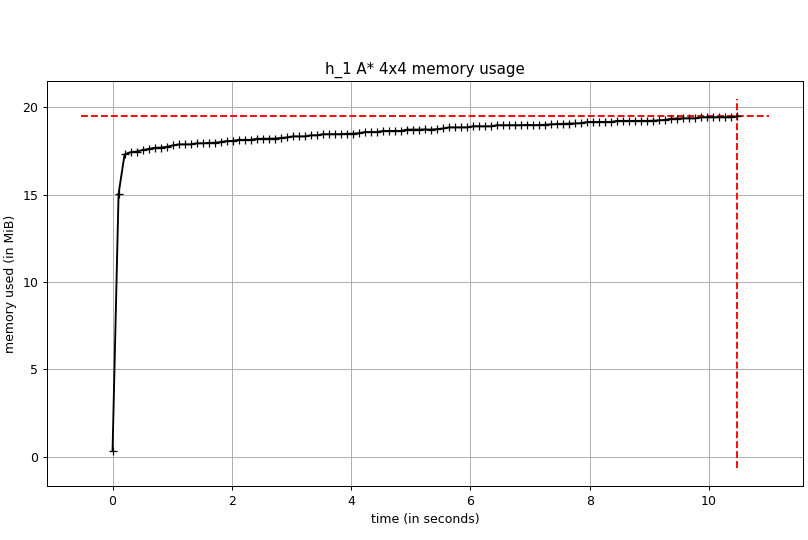
\includegraphics[width=10cm]{images/a_star_h1_4x4.png}
        \caption{Memory usage of A* under $h_1$} \label{fig2}
    \end{center}
\end{figure}
    
\begin{figure}
    \begin{center}
        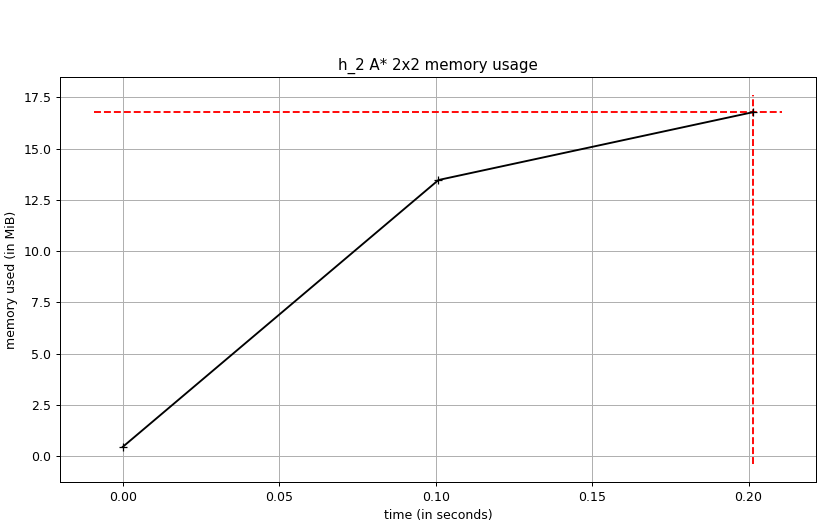
\includegraphics[width=10cm]{images/a_star_h2_2x2.png}
        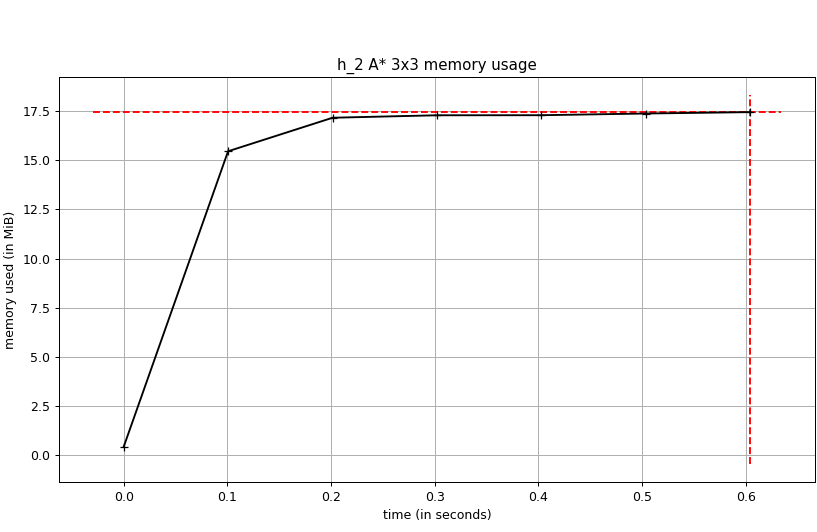
\includegraphics[width=10cm]{images/a_star_h2_3x3.png}
        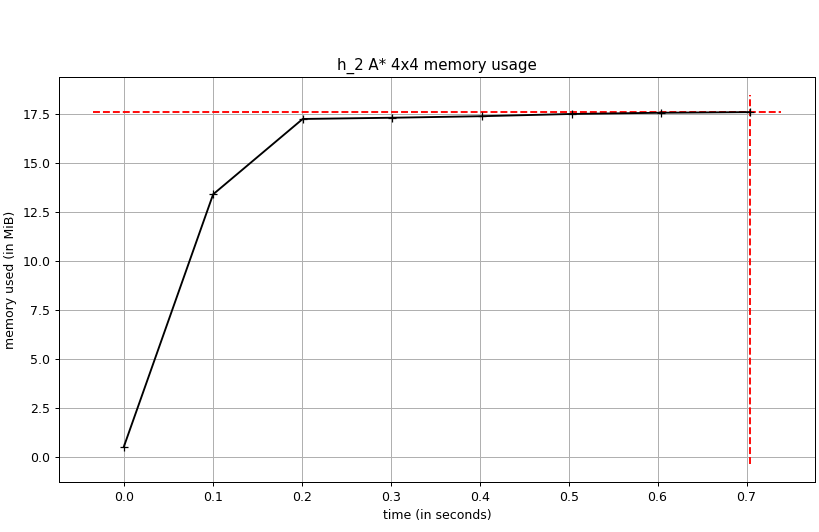
\includegraphics[width=10cm]{images/a_star_h2_4x4.png}
        \caption{Memory usage of A* under $h_2$} \label{fig3}
    \end{center}
\end{figure}
    
\newpage

\subsection{Appendix B - Search and Solution Paths}

\begin{figure}
    \begin{center}
    \begin{BVerbatim}
    0 0 0 1010010111001010
    0 0 0 0110110111001010
    0 0 0 1010010111001010
    0 0 0 0110110111001010
    0 0 0 1010010111001010
    0 0 0 0110110111001010
    0 0 0 1010010111001010
    0 0 0 0110110111001010
    0 0 0 1010010111001010
    0 0 0 0110110111001010
    ...
    0 0 0 0000001010110000
    0 0 0 0000000111110011
    0 0 0 0000000001001110
    0 0 0 0000000010001100
    0 0 0 0000000011100101
    0 0 0 0000000011010001
    0 0 0 0000000000000000
    \end{BVerbatim}
    \caption{Search path output of dfs on 4x4 test case.}
    \end{center}
\end{figure}

\begin{figure}
    \begin{center}
    \begin{BVerbatim}
    2 0 2 1010010111001010
    3 1 2 0010100101001010
    3 2 1 0001100001001010
    3 2 1 0010000110000010
    3 2 1 0010100100000100
    3 1 2 0100000111001010
    3 2 1 0100000101000110
    3 2 1 0100000110000100
    3 2 1 0100100100000010
    3 1 2 0110110111001010
    3 2 1 0110010100000010
    ...
    4 2 2 0110111110111000
    4 3 1 0111000010000100
    4 2 2 0111000011001010
    4 3 1 0111100000000010
    4 3 1 1000000000010100
    4 3 1 1000000010001011
    4 3 1 1000000100000010
    4 3 1 1000001000101000
    4 2 2 1000001001100110
    4 3 1 1000001001000001
    4 3 1 1000001010000011
    \end{BVerbatim}
    \caption{Search path output of A* under $h_1$ on 4x4 test case. The third number represents the value of $g(s)$} \label{fig10}
    \end{center}
    \end{figure}
    
    \begin{figure}
    \begin{center}
    \begin{BVerbatim}
    8 0 8 1010010111001010
    7 1 6 0010100101001010
    6 2 4 0010000110000010
    6 3 3 0001000010000010
    6 2 4 0010100100000100
    6 3 3 0001100000000100
    7 2 5 0001100001001010
    7 1 6 0100000111001010
    6 2 4 0100000110000100
    6 3 3 0100000100001000
    6 2 4 0100100100000010
    6 3 3 1000000100000010
    7 2 5 0100000101000110
    7 1 6 1010010110000100
    7 2 5 1000001010100100
    7 3 4 1000001000101000
    7 3 4 1000011001000000
    7 2 5 1001010010000100
    7 3 4 1001000001100000
    7 3 4 1001010000001000
    7 2 5 1010000101100000
    7 2 5 1010010100001000
    7 1 6 1010110100000010
    7 2 5 0110010100000010
    7 3 4 0100001000100010
    7 4 3 0100000001010000
    7 3 4 0101010000000010
    7 2 5 1000101000100010
    7 3 4 1000100001010000
    7 2 5 1001110000000010
    7 4 3 1100100000000000
    5 5 0 0000000000000000
    \end{BVerbatim}
    \caption{Search path output of A* under $h_2$ on 4x4 test case. The third number represents the value of $g(s)$} \label{fig2}
    \end{center}
    \end{figure}
    


\end{document}

